\begin{table}[t]
\centering
\begin{tabular}{|c|l|}
\hline
App & \multicolumn{1}{c|}{Invariants}\\\hline
TPC-W & $\forall \mathit{item} \in \mathit{item\_table}.~\  \mathit{item}\ldotp\mathit{stock} \geq 0$ \\\hline
\multirow{3}{*}{RUBiS} & $\forall \mathit{item} \in \mathit{item\_table}.~\ \mathit{item}\ldotp\mathit{quantity} \geq 0$\\
\cline{2-2}
& $\forall u, v \in \mathit{user\_table}.~$ \\
& $\quad u\ldotp\mathit{uname} = v\ldotp\mathit{uname} \implies u = v$\\\hline
\end{tabular}
\caption{Application-specific invariants}
\label{tab:staticinvariants}
\end{table}

\section{Evaluation}
\label{ch:sieve:sect:evaluation}
In this section, we report our experience with implementing \tool,
adapting existing web applications to run with \tool, and evaluating
these systems.

\subsection{Implementation}
We implemented most of our tool using Java (15k lines of code), and changed parts of the Jahob code
to obtain weakest preconditions in OCaml (553 lines of code)~\footnote{The lines of code is
measured by {\tt cloc}~\cite{codecounter}.}. The
backend storage system we used was a MySQL database. We used
an existing Java parser~\cite{javaparser} to parse java files for generating an
abstract syntax tree (AST). Finally, we connected our tool
to the Gemini replication and coordination system, as presented in Section~\ref{ch:redblue:sect:gemini}, to enable both
consistency classification and operation replication. The sourcecode is available at ~\cite{SIEVESource}.

\subsection{Use cases}
To adapt an application to use \tool, one has to annotate the
corresponding SQL schema with the proper CRDT semantics, specify
all invariants, and finally the original JDBC driver must be replaced
by the driver provided by \tool, to enable
\tool\ to intercept interactions between the application and the database.

We applied \tool\ to two web application benchmarks, namely TPC-W~\cite{TPC-Wv18}
and RUBiS~\cite{RUBiS}. Both of them simulate an online
store and the interactions between users and the web application. 
There are two main motivations for selecting these use cases: (1)
both have been widely used by the community to evaluate system performance; and
(2) both have application-specific invariants that can be violated 
under causal consistency. We recall the
invariants of these two applications in Table~\ref{tab:staticinvariants}. 
(In Chapter~\ref{chapter:redblue},
a social application is evaluated, but it made no sense to 
include this application because it
did not contain any invariants that could be violated under weak consistency.)

For TPC-W, we use \texttt{AOSET}, \texttt{AUSET}, \texttt{UOSET} and
\texttt{ARSET}, as specified in Table~\ref{tab:crdts}, to annotate the database tables,
no annotations for unmodified attributes, \texttt{NUMDELTA}
for \texttt{stock}, and \texttt{LWW} for the remaining attributes. For
RUBiS, we annotate its tables with \texttt{AUSET} and \texttt{AOSET}.
We use \texttt{NUMDELTA} as annotations for both \texttt{quantity} ({\tt stock}) and \texttt{numOfBids}, and
no annotations or \texttt{LWW} for the remaining attributes. For additional details, we refer the interested reader to the code available in~\cite{SIEVESampleData2014}.

In terms of the time required to do this adaptation, we do not report results
for TPC-W as we relied on this use case during the design and development phase
of \tool. However for the RUBiS use case, the entire process
was concluded in only a few hours.
An interesting point to highlight is that \tool\ is
able to detect inconsistencies between these annotations \changebars{such as
tagging a table as update-only ({\tt UOSET}) but the original code contains insert
sql commands against that table }{}, enabling
programmers to  correct  mistakes such as type omissions in the SQL schema
that are inconsistent with the CRDT annotations.

In both the RedBlue consistency framework~\ref{chapter:redblue} and SIEVE,
the effort we made analyzing application code to determine
invariants and merge semantics is unavoidable. 
In the former case, however,
we additionally spent a significantly larger amount of time manually implementing 
merge semantics, and classifying shadow operations by taking into account their
properties, for every application. \tool\ eliminates
all this manual work, and limits human error.

\subsection{Experimental setup}
All reported experiments were obtained by deploying applications on a local cluster,
where each machine has
2*6 i7 cores and 48GB RAM, and runs Linux 3.2.48.1 (64bit), MySQL 5.5.18,
Tomcat 6.0.35, and Java 1.7.0. The reason we did not include
geo-distributed experiments is that we wanted
to extensively focus on evaluating various aspects of \tool, instead of
performance benefits enhanced by RedBlue consistency, which are already
shown in Section~\ref{ch:redblue:sect:eval}.

\subsection{Experimental results}
Our experimental work aims at evaluating both the static analysis component of \tool\ and also 
the runtime component, which includes a performance
comparison between each application using our tool, its unmodified version, and
its version under RedBlue consistency where the entire classification
is done manually and offline.

Concerning the static analysis component we focus on the following main questions: 
%$(i)$ What are the outputs generated by the static analysis component?
\begin{enumerate}
\item How long does the static analysis process take to complete?
\item What is the scalability of the static analysis component in relation to the size of the code base?
\end{enumerate}

For the runtime component of \tool\ we focus on the following main questions: 
\begin{enumerate}
\item Is the runtime classification of shadow operations accurate?
\item What is the (runtime) overhead for adapted applications compared to their stand-alone unmodified counterparts?
\item What are the performance gains obtained through weakly consistent replication using \tool?
\end{enumerate}
\begin{table*}[t!]
\small
\centering
\subfloat[TPC-W]{
\begin{tabular}{|l|c|c||l|c|c|}
\hline
 Transaction name & \#paths & \#templates & Transaction name & \#paths & \#templates\\
\hline
createEmptyCart & 1 & 1 & getRelated & 1 & 0\\
doCart & 36 & 36 & getNewProducts & 1 & 0 \\
GetMostRecentOrder & 1 & 0 & createNewCustomer & 2 & 2\\
adminUpdate & 4 & 4 & getBestSellers & 1 & 0 \\
getName & 1 & 0 & doAuthorSearch & 1 & 0 \\
doSubjectSearch & 1 & 0 & GetPassword & 1 & 0\\
doTitleSearch & 1 & 0 & refreshSession & 1 & 1 \\
GetUserName & 1 & 0 & getCustomer & 1 & 0\\
getCart & 1 & 0 & doBuyConfirm-A & 32 & 32 \\
doBuyConfirm-B & 16 & 16 & getBook & 1 & 0 \\
\hline
\end{tabular}
\label{tab:staticanalysistpcwpath}
}
% \subfloat[TPC-W]{
% \centering
%  \begin{tabular}{|l|c|c||l|c|c|}
% \hline
%   Transaction name & \#paths & \#templates & Transaction name & \#paths & \#templates\\
% \hline
% read-only txns (13) & 1 & 0 &  createNewCustomer & 2 & 2 \\
% refreshSession & 1 & 1 & createEmptyCart & 1 & 1 \\
% adminUpdate & 4 & 4 & doCart & 36 & 36\\
% doBuyConfirm-A & 32 & 32 &  doBuyConfirm-B & 16 & 16\\
% \hline
%  \end{tabular}
% \label{tab:staticanalysistpcwpath}
% }

%\vspace{3mm}
\subfloat[RUBiS]{
\begin{tabular}{|l|c|c||l|c|c|}
%{|p{3.55cm}|c|c||p{2.6cm}|c|c|}%{|p{3.3cm}|c|c|}
\hline
Transaction name & \#paths & \#templates & Transaction name & \#paths & \#templates\\
\hline
ViewUserInfo & 6 & 0 & PutComment & 10 & 0\\
PutBid & 14 & 0 & BrowseRegions & 5 & 0 \\
StoreComment & 11 & 3 & StoreBid & 17 & 5 \\
BuyNow & 7 & 0 & ViewBidHistory & 11 & 0 \\
AboutMe & 37 & 0 & ViewItem & 10 & 0 \\
StoreBuyNow & 13 & 6 & RegisterItem & 59 & 24\\
SearchItemsByCategory & 20 & 0 &  BrowseCategories & 13 & 0\\       
SearchItemsByRegion & 20 & 0 & RegisterUser & 14 & 3\\
\hline
\end{tabular}
\label{tab:staticanalysisrubispath}
}

\caption{Number of reduced paths and templates generated for each transaction in TPC-W and RUBiS.}
    \label{tab:staticanalysispathreducetpcw}
\end{table*}

\subsubsection{Static analysis}
As mentioned before, taking the application source code and CRDT annotations as input, \tool\
first maps each transaction into a set of distinct paths, and automatically transforms each path into a shadow operation template. 


Table~\ref{tab:staticanalysispathreducetpcw}
summarizes the number of paths (excluding loops) and the corresponding number of shadow operation templates that were produced by \tool\ for
both TPC-W and RUBiS. For TPC-W, $15$ out of the total $20$ transactions only exhibit
a single path, as the code of these transactions is sequential. The two most complex transactions in this use case are
\texttt{doBuyConfirm} and \texttt{doCart}, which are associated with the user actions of
shopping and purchasing.
In contrast, most transactions in RUBiS have a more complex control flow,
which generated a larger number of possible execution paths. 

Note that the majority of transactions in both use cases do not lead \tool\ to
produce any template. This happens when the transactions are read-only, and therefore do not have side effects. Additionally, in TPC-W every path in an update transaction
generates a shadow operation template, since system state is always modified. However, this is 
not true in RUBiS, because its code verifies several conditions, some of which lead to a read-only transaction. 
%an abort.
\begin{table}[t!]
\centering
    \begin{tabular}{ | c | c | c | c | c | c |}
    \hline
    \multirow{2}{*}{App} & \multirow{2}{*}{\#code} & \multicolumn{2}{c|}{templates} & \multirow{2}{*}{\#db code} & \multirow{2}{*}{\#specs}\\ \cline{3-4}
       &       &  num & \#code & & \\\hline
    TPC-W & 8.3k & 92 & 1554 & 879 & 730\\
    RUBiS & 9.8k & 41 & 251 & 477 & 371\\
    \hline
    \end{tabular}
    \caption{Overview of the output produced by the static analysis. ``db code'' refers to the Java classes representing  database structures required for computing weakest preconditions.}
    \label{tab:staticanalysisoutput}
\end{table}

\begin{table}[t!]
\centering
\begin{tabular}{|c|c|c|}
\hline
 & WP & Comments \\
\hline
\multirow{2}{*}{TPC-W} & \texttt{TRUE} & Not influencing invariants \\
\cline{2-3}
& $\texttt{delta} \geq 0$ & Non-negative stock \\
\hline
\multirow{4}{*}{RUBiS} & \texttt{TRUE} & Not influencing invariants \\
\cline{2-3}
& \texttt{FALSE} & Nickname must be unique \\
\cline{2-3}
& $\texttt{delta} \geq 0$ & Non-negative quantity \\
\cline{2-3}
& $\texttt{quantity} \geq 0$ & Non-negative quantity (new item) \\
\hline
\end{tabular}
\caption{Weakest preconditions (WP)}
\label{tab:generatedwp}
\end{table}

\begin{table}[t!]
\centering
\begin{tabular}{|c|c|c|c|c|}
\hline
App & JahobSpec & Template & WP & Total \\\hline
TPC-W & 9.1 $\pm$ 0.1 & 3.8 $\pm$ 0.1 & 3.3 $\pm$ 0.1 & 16.2 $\pm$ 0.3 \\
RUBiS & 8.9 $\pm$ 0.0 & 3.3 $\pm$ 0.3 & 0.9 $\pm$ 0.1 & 13.2 $\pm$ 0.3 \\
\hline
\end{tabular}
\caption{Average and standard deviation of latency in seconds for static analysis tasks (5 runs).}
\label{tab:timestatic}
\end{table}

As depicted in Table~\ref{tab:staticanalysisoutput}, the execution
of \tool\ generated a total of $92$ and $41$ shadow operation
templates for TPC-W and RUBiS, respectively.  In addition to these
templates, our tool also generates automatically a set of Java classes
that represent database data structures, which are necessary
for computing weakest preconditions.
%%alongside specific logic conditions that are used by Jahob.

\begin{figure}[t!]
\centering
\subfloat[TPC-W]{
\centering
%\begin{minipage}[b]{0.45\textwidth}
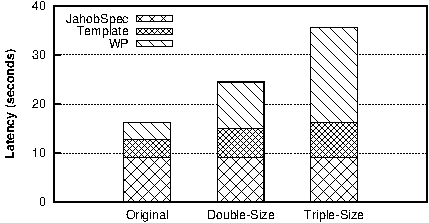
\includegraphics[width=0.66\textwidth]{./figures/sieve/eval/xytpcwanalysis.pdf}
\label{fig:tpcwtimeanalysis1}
%\end{minipage}
}
\par\bigskip
\subfloat[RUBiS]{
\centering
%\begin{minipage}[b]{0.45\textwidth}
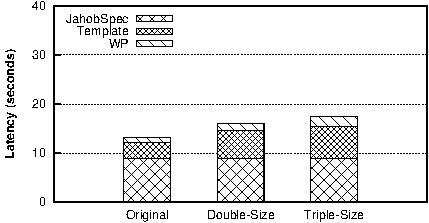
\includegraphics[width=0.66\textwidth]{./figures/sieve/eval/xyrubisanalysis.pdf}
\label{fig:rubistimeanalysis1}
%\end{minipage}
}
\caption{Static analysis time vs.\ code base size.}
\label{fig:compDiffSize}
\end{figure}

Table~\ref{tab:generatedwp} depicts a full list of the different weakest preconditions
generated by \tool\ for both use cases. These weakest preconditions alongside their 
respective shadow operation template identifiers are used by the runtime logic to classify shadow operations as either blue or red. 
A weakest precondition denoted by \texttt{TRUE} implies that any shadow operation associated
with that template is always invariant safe and therefore labeled blue.
In contrast, a weakest precondition denoted by \texttt{FALSE} implies that shadow operations
associated to that template must always be classified as red.
The remaining non-trivial conditions must be evaluated at runtime by replacing their 
arguments with concrete values. For
instance, when a \texttt{doBuyConfirm} transaction produces a negative delta, then
the condition will be evaluated to \texttt{FALSE} and the corresponding shadow operation will
be classified as red, otherwise the condition will be evaluated to \texttt{TRUE} and the 
shadow operation will be classified as blue.

\paragraph{Cost of static analysis.} A relevant aspect of the static analysis component
in \tool\ is the time required to execute it. To study this we have measured the time
taken by the static analysis and present the obtained results in Table~\ref{tab:timestatic}.
We not only measured the end-to-end completion time, but also the time
spent for each step, namely, creating database data structures required by Jahob (JahobSpec), 
template creation (Template), and weakest precondition computation (WP). 
Overall, we can see that the execution time
of the static component of \tool\ is acceptable, as less than
20 seconds are required to analyze both TPC-W and RUBiS. 
%The weakest precondition
%computation via Jahob dominates the overall static analysis time. 
The code generation phase including both JahobSpec and Template dominates
the overall static analysis. Compared to TPC-W, the time spent
computing weakest preconditions is shorter in RUBiS, due to
the smaller number of templates in Table~\ref{tab:staticanalysisoutput}.
%Compared
%to TPC-W, the time spent extracting path information in RUBiS is larger, due to
%the more complex control flow of RUBiS, as shown in Table~\ref{tab:staticanalysistpcwpath}.

%\begin{table*}[!ht]
%\footnotesize
%\centering
%\begin{tabular}{|c|c|c|c|c|c|c|}
%\hline
%App & CFG & PathAb & ReducedPathAb & Template & WP & Total \\\hline
%TPC-W & 460.5 $\pm$ 110.8 & 292.1 $\pm$ 22.2 & 365.9 $\pm$ 29.4 & 294.0$\pm$ 168.9 & 3519.6 $\pm$ 156.2 & 4932.1 $\pm$ 184.8\\
%RUBiS & 309.1 $\pm$ 75.9 & 656.0 $\pm$ 44.1 & 501.0 $\pm$ 27.2 & 248.4 $\pm$ 42.9 & 841.1 $\pm$ 41.2 & 2555.5 $\pm$ 174.0\\
%\hline
%\end{tabular}
%\caption{Average latency in milliseconds plus standard deviation for static analysis tasks (5 runs).}
%\label{tab:timestatic}
%\end{table*}

\paragraph{Scalability.} The code base size of TPC-W and RUBiS is somewhat
small when compared to deployed applications.  This raises a question
concerning the scalability of the static analysis component of
\tool\ with respect to the size of the code base. In order to analyze this aspect of \tool\ 
we have artificially doubled and tripled the size of each application
code base and measured the time spent analyzing these larger
code bases when compared with the original. The results are shown in
Figure~\ref{fig:compDiffSize}. The time spent generating the
data structures required by Jahob is constant, since we did not
change the database schema. However, the time spent
computing the weakest preconditions for templates in TPC-W grows
exponentially, and the time taken for the remaining steps presents a
sub-linear increase. These results lead us to conclude
that the static analysis of \tool\ may scale to reasonable though not very large code sizes,
especially taking into account that this process is executed a single
time when adapting an application through the use of \tool.


\subsubsection{Runtime logic}
We evaluated the runtime performance of our example
applications using \tool\ on top of Gemini.
% which is a
%coordination and replication layer supporting generator
%and shadow operation execution~\cite{Li2012RedBlue}.
%To evaluate the performance overheads of  \tool, we compare it to a 
%non-automated solution, in which we manually created
%shadow operations, and classified them by analyzing the code ourselves
%to see if it meets the conditions defined in~\cite{Li2012RedBlue}.

%%Due to this, we start by first studying the introduced overhead, and then we focus on
%%the performance benefits that can be achieved by employing \tool\ to replicate these applications. 

%% To address the overhead study we conduct a performance study where we compare the 
%% performance of the original un-replicated use cases against the their manual
%% adaptation to operate under red-blue consistency (dubbed Manual, which follows the strategy
%% presented in~\cite{Li12RedBlue}) and their automatic adaptation using \tool\ on a single site
%% deployment. We then follow with a performance study in a replicated scenario with two replicas 
%% where we measure the latency and throughput achieved for the un-replicated
%% use cases, agains both the manual and automatic (\tool) adaptation of these use cases.

%% However, as a first step we start by verifying that the classification of shadow operations
%% performed by \tool\ is correct, meaning that only invariant-preserving shadow operations
%% are labelled blue. And also we verify that only non-invariant-preserving shadow operations
%% are labelled red.

\paragraph{Configurations.}  We populated the dataset for TPC-W using the
following parameters: 50 EBS and 10,000 items. For RUBiS we populated
the dataset with 33,000 items for sale, 1 million users, and 500,000
old items. We exercised all TPC-W workloads, namely browsing mix,
shopping mix, and ordering mix, where the purchase activity varies
from 5\% to 50\%. For RUBiS, we ran the bidding mix workload, in which
15\% of all user activities generate updates to the application state.
% 
% 
% {\bf Classification accuracy.}
% We start by verifying that the classification of shadow operations
% performed by \tool\ is correct, meaning that operations are labeled blue if and
% only if they are
% invariant-preserving.

\begin{table}[t!]
\centering
    \begin{tabular}{ | c | c | c | c |}
    \hline
    App & Workload & Manual & \tool\\\hline
    \multirow{3}{*}{TPC-W} & Browsing mix & 0.49 ($\pm$ 0.03) & 0.48 ($\pm$ 0.02) \\
                 & Shopping mix & 0.79 ($\pm$ 0.02) & 0.81 ($\pm$ 0.02) \\
                 & Ordering mix & 6.31 ($\pm$ 0.04) & 6.30 ($\pm$ 0.07) \\
    \hline
    RUBiS & Bidding mix & 2.65 ($\pm$ 0.09) & 2.62 ($\pm$ 0.07)\\
    \hline
    \end{tabular}
    \caption{Percentage of red shadow operations classified manually and by \tool\ (5 runs).}
    \label{tab:classfyresult}
\end{table}

\begin{figure}[t!]
\centering
\subfloat[TPC-W shopping mix]{
\centering
%\begin{minipage}[b]{1.0\textwidth}
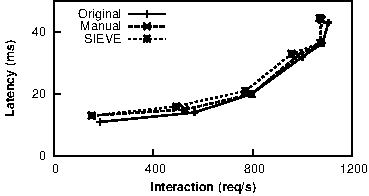
\includegraphics[width=0.85\textwidth]{./figures/sieve/eval/thlatpcw1dc.pdf}
\label{fig:thputLatencyTPCW}
%\end{minipage}
}
\par\bigskip
\subfloat[RUBiS bidding mix]{
\centering
%\begin{minipage}[b]{1.0\textwidth}
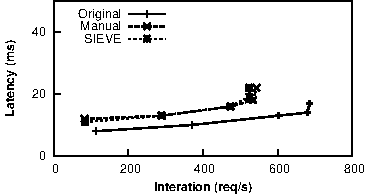
\includegraphics[width=0.85\textwidth]{./figures/sieve/eval/thlarubis1dc.pdf}
\label{fig:thputLatencyRUBiS}
%\end{minipage}
}
\caption{Throughput-latency graph without replication}
\label{fig:evalThroughputLatency}
\end{figure}

\paragraph{Correctness validation.} To verify that \tool\ labels operations correctly for
both case studies, we compared  the classification results
obtained by running \tool\ with TPC-W and RUBiS against
the results achieved manually in Chapter~\ref{chapter:redblue}.
Our finding in Table~\ref{tab:classfyresult} shows that
the percentage of shadow operations classified as red by \tool\ 
matches the results obtained through the manual classification.
In addition, a careful inspection of the logs shows that the expected pairs of functions and parameters 
were in fact labeled as red. This implies that \tool\ is able to achieve the same 
labeling as a manual process while saving a significant amount of effort from 
programmers and avoiding human mistakes.
% the log files generated by running
% \tool\ with TPC-W and RUBiS, and we found that \tool\ conducts the same 
% classification that was achieved manually in our previous work.
%  summarizes the classification results
% obtained both through manual classification and \tool.  
\begin{figure}[t!]
\centering
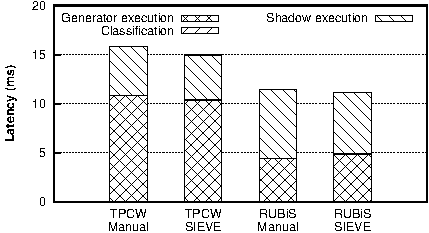
\includegraphics[width=0.85\textwidth]{./figures/sieve/eval/latencyBreakDownBar1.pdf}
\caption{Breakdown of latency.}
\label{fig:latencybreakdownbar}
\end{figure}

\paragraph{\tool\ runtime overhead.} Next we compared the performance
(throughput vs.\ latency) of the two applications across three
single-site deployments: 1) \tool, 2) Original---the original unreplicated
service without any overheads from creating and applying shadow
operations, and 3) Manual---the RedBlue scheme with all labeling
performed offline by the programmer. The expected sources of overhead
for \tool\ are: $i)$ the dynamic creation of shadow operations; and
$ii)$ the runtime classification of each shadow operation.  The
results in Figure~\ref{fig:evalThroughputLatency} show that the
performance achieved by \tool\ is similar to the one obtained with a
manual classification scheme, and therefore the overheads of runtime
classification are low. The comparison with the original scheme in a
single site shows some runtime overhead due to creating and applying
shadow operations (which is required for a replicated deployment so
that all operations commute).
%Also these results validate our expectations that the runtime overhead imposed by our
%mechanisms is negligible when compared with the unmodified use cases.

To better understand the sources of overhead imposed by \tool\ we
measured the latency contribution of each runtime step executed
by \tool\ and compared it with the latency contribution of these steps when relying on a manual
adaptation. In particular, we focused on the following tasks: generator execution (producing a shadow operation), classification (determining
shadow operation colors), and shadow execution (applying shadow operations). 

Figure~\ref{fig:latencybreakdownbar} shows the average contribution to request latency of
each of these steps (Only update requests are considered
since read-only queries do not generate side effects.) For the manual adaptation, there is no latency associated with classifying shadow operations, 
since the classification of all shadow operations is pre-defined. In contrast,
\tool\  performs a runtime classification, but the results show that the time consumed in this task is negligible. 
In particular,
% this takes is instantaneous (zero latency contribution) to
%verify weakest preconditions of read-only shadow operation (which are trivially blue). 
%for update shadow operations,
 \tool\ takes 0.064 $\pm$ 0.002 $ms$ and
0.072 $\pm$ 0.001 $ms$ for looking up the dictionary and evaluating
the condition for TPC-W and RUBiS, respectively. Regarding the
generator execution and shadow execution, both the manual adaptation and \tool\ present
the same latency overheads.


\if 0
Figure~\ref{fig:rubislatencybar} shows the average latency of every single interaction from
all deployments, namely original RUBiS, RUBiS with Gemini, and RUBiS
with \tool. From the results, we conclude that the overhead introduced by \tool\ is
very small. As shown in Figure~\ref{fig:rubislatencybar1}, \tool\ doesn't
add extra latency to each read-only interaction. The reason is that \tool\ will not
generate a shadow operation for any read-only transaction, and will not invoke
weakest precondition checking as well. As shown in Figure~\ref{fig:rubislatencybar2},
we add a small amount overhead to the updating interaction, but not much. Gemini manually
defines a set of shadow operation classes, and classify these classes as Red or Blue, statically.
Despite this, in order to create an instance to instantiate these classes, one using Gemini
has to inject codes inside applications to keep track of updates, and encode these updates into
the created instances. This part is as the same as what we are doing with \tool. The only difference
is that Gemini doesn't need runtime evaluation, but \tool\ does. However, the evaluation is 
lightweight.

\begin{figure*}[!ht]
\centering
\subfloat[Read-only interaction]{
%\begin{minipage}[b]{0.5\textwidth}
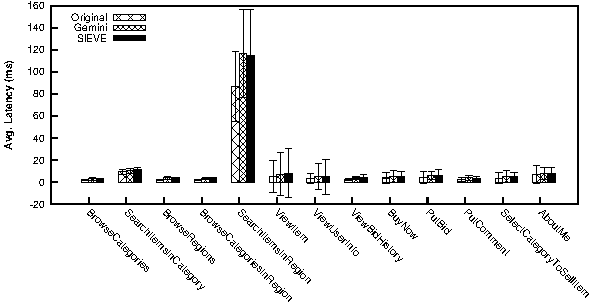
\includegraphics[height=0.33\textheight]{./figures/sieve/eval/rubisLatencyBarReadonly.pdf}
\label{fig:rubislatencybar1}
%\end{minipage}
}
\par\bigskip
%\hspace{0.4cm}
\subfloat[Update interaction]{
%\begin{minipage}[b]{0.5\textwidth}
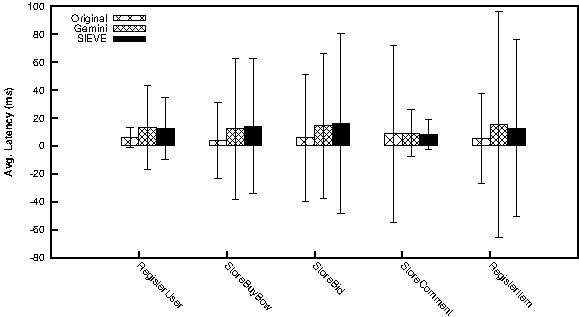
\includegraphics[height=0.33\textheight]{./figures/sieve/eval/rubisLatencyBarWrite.pdf}
\label{fig:rubislatencybar2}
%\end{minipage}
}
\caption{Average latency of different iterations. For other iterations
that don't have database access, the difference is negligible, so we
don't put into the figure.}
\label{fig:rubislatencybar}
\end{figure*}

Figure~\ref{fig:tpcwlatencybar} shows the comparison of the average
latency per interaction across three different deployments.

\begin{figure*}[!ht]
\centering
\subfloat[High latency]{
%\begin{minipage}[b]{0.5\textwidth}
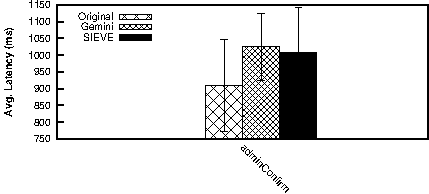
\includegraphics[height=0.33\textheight]{./figures/sieve/eval/tpcwLatencyBarhigh.pdf}
\label{fig:tpcwlatencybar1}
%\end{minipage}
}
%\hspace{0.4cm}
\par\bigskip
\subfloat[Low latency]{
%\begin{minipage}[b]{0.5\textwidth}
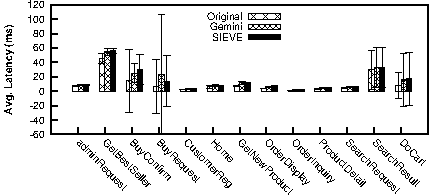
\includegraphics[height=0.33\textheight]{./figures/sieve/eval/tpcwLatencyBarlow.pdf}
\label{fig:tpcwlatencybar2}
%\end{minipage}
}
\caption{Average latency of different interactions. \cheng{The Gemini curve uses
the same data as SIEVE, since the data is not available now and my script
to build this chart requires three inputs.}}
\label{fig:tpcwlatencybar}
\end{figure*}
\fi

%\allen{Important graph/experiment that is missing is the comparison to
%  the hand-tuned implementations from OSDI.  Have we introduced
%  excessive overheads?}

\begin{figure}[t!]
\centering
\subfloat[TPC-W shopping mix]{
%\begin{minipage}[b]{0.5\textwidth}
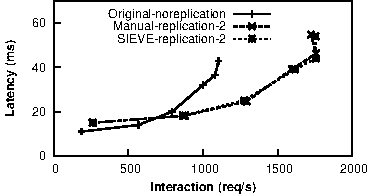
\includegraphics[width=0.86\textwidth]{./figures/sieve/eval/thlatpcwall.pdf}
\label{fig:thputLatencyTPCWRep}
%\end{minipage}
}
\par\bigskip
\subfloat[RUBiS bidding mix]{
%\begin{minipage}[b]{0.5\textwidth}
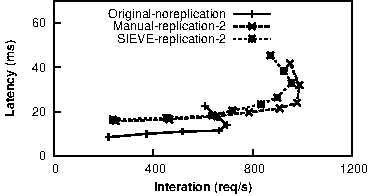
\includegraphics[width=0.86\textwidth]{./figures/sieve/eval/thlarubisall.pdf}
\label{fig:thputLatencyRUBiSRep}
%\end{minipage}
}
\caption{Throughput-latency graph with two replicas.}
\label{fig:evalThputLatency}
\end{figure}

\paragraph{Replication benefits.}
The results previously discussed in this section have shown that the
use of \tool\ imposes a small overhead when compared to a standalone
execution of the unmodified use cases, mostly due to runtime
classification. However, \tool\ was designed to allow replication to
bring performance gains through the use of weak consistency in
replicated deployments. To evaluate these benefits, we conducted an
experiment where we deployed the two applications (1) without
replication, (2) using manual classification in Gemini, and (3)
using \tool, with two replicas in the same site for the last two
options. (The use of single site replication instead of
geo-replication makes our results conservative, since the overheads of
runtime classification become diluted when factoring in cross-site
latency.) 

The results in Figure~\ref{fig:evalThputLatency} show that weakly consistent replication for a large
fraction of the operations brings performance gains. In particular, one
observes that the peak throughput with 2 replicated Gemini instances
running TPC-W is improved by 59.0\%, and the peak throughput for
RUBiS in this setting is improved by 37.4\%. %raw number (955-695)/695
The additional latency
introduced in this case is originated by the necessity of coordination
among replicas to totally order red shadow operations. The results
also confirm that the overhead of runtime classification when compared
to the manual, offline classification are low. Note that there is a
point where the throughput goes down while there is still an increase
in latency in Figure~\ref{fig:evalThputLatency}\subref{fig:thputLatencyRUBiSRep}. This happens
because the database becomes saturated at this point.

